%%%%%%%%%%%%%%%%%%%%%%%%%%%%%%%%%%%%%%%%%%%%%%%%%%%%%%%%%%%%%%%%%%%%%%
%     File: ExtendedAbstract_resul.tex                               %
%     Tex Master: ExtendedAbstract.tex                               %
%                                                                    %
%     Author: Andre Calado Marta                                     %
%     Last modified : 27 Dez 2011                                    %
%%%%%%%%%%%%%%%%%%%%%%%%%%%%%%%%%%%%%%%%%%%%%%%%%%%%%%%%%%%%%%%%%%%%%%
% Results
% Results should be clear and concise.
% Discussion
% This should explore the significance of the results of the work, not
% repeat them. A combined Results and Discussion section is often
% appropriate. Avoid extensive citations and discussion of published
% literature.
%%%%%%%%%%%%%%%%%%%%%%%%%%%%%%%%%%%%%%%%%%%%%%%%%%%%%%%%%%%%%%%%%%%%%%

\section{Results}
\label{sec:resul}
In this section, the dataset used is described and the results obtained are presented. First, the descriptive statistics are provided, then the DEA scores are obtained, followed by the truncated regression analysis, and finally the Malmquist index results.
\subsection{Dataset description}
\label{subsec:resul_data}
Our dataset includes 41 Iberian airports, including 5 in Portugal and 36 in Spain, over a period of eight years (2016-2023). Following the airport size definition from \cite{ripoll-zarraga2020}, \figref{fig:mapa} displays a map with the geographical location of the airports and their respective sizes.  


\begin{figure}[h!]
  \centering
  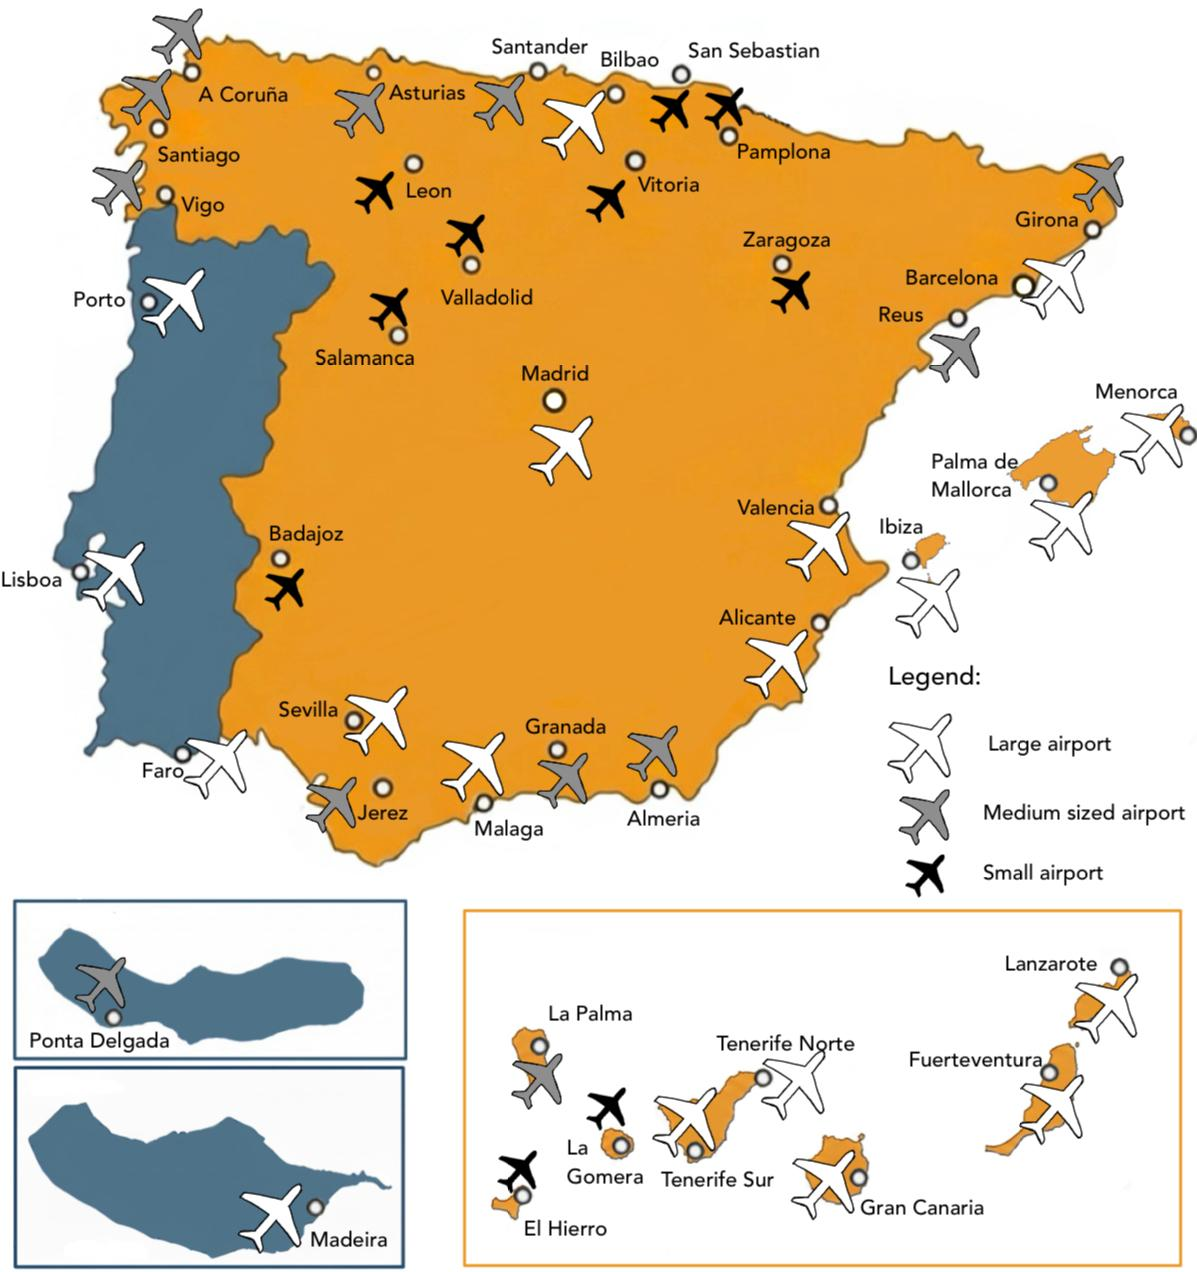
\includegraphics[width=8cm]{images/mapa.jpg}
  \vspace{-0.5cm}
  \caption{Location and size classification of the 41 Iberian airports}
  \label{fig:mapa}
\end{figure}

DEA models require the identification of the inputs and outputs of the analysis. As DEA is not a
statistical technique, there is no systematic approach for the selection of inputs and outputs, therefore the first practical criterion for selecting these
variables is data availability. \tabref{tab:variables} lists these variables
and summarizes their main descriptive statistics, namely the minimum (Min.), maximum (Max.), mean,
and standard deviation (St. Dev.) values.


\begin{table}[h!]
  \begin{center}
    \caption{Summary Statistics for Input and Output Variables (2016–2023)}
    \label{tab:variables}
    \resizebox{\columnwidth}{!}{%
  \begin{tabular}{lcccc}
        \toprule
        \textbf{Variables} & \textbf{Min.} & \textbf{Max.} & \textbf{Mean} & \textbf{St. Dev.} \\
        \midrule
        \multicolumn{5}{l}{\textit{Inputs}} \\
       Employees & 17 & 42,222 & 3,409 & 7,862 \\
         Runway \\Area
    ($m^2$) & 37,500 & 910,020 & 169,293 & 142,191 \\
        Gates & 2 & 238 & 24.8 & 42.4 \\
        \midrule
        \multicolumn{5}{l}{\textit{Outputs}} \\
         Passengers & 2,358 & 61,652,021 & 6,437,865 & 11,112,114 \\
        ATM & 1,086 & 426,324 & 53,780 & 76,780 \\
         Cargo (t) & 0 & 655,586 & 27,546 & 89,429 \\
        \bottomrule
 \end{tabular}%
    }
  \end{center}
\end{table}
  \vspace{-0.5cm}
Even though this selection of input variables does not fully
represent the most common variables in the literature review conducted in \autoref{sec:backg} due to data availability constraints, it is still in line with the previous literature.

It is important to highlight that only physical measures of capital were considered in this analysis. This
approach was necessary since airport-level financial data stopped being published, following Aena’s partial privatization in 2014.

Regarding the second-stage regression, \tabref{tab:exp_statistics} lists the explanatory variables used in the second-stage regression to explain DEA efficiency scores.


\begin{table}[h!]
  \begin{center}
        \caption{Summary Statistics for explanatory variables}
    \label{tab:exp_statistics}
    % Define centered column type
   \resizebox{\columnwidth}{!}{%
  \begin{tabular}{lcccc}
        \toprule
        \textbf{Explanatory Variables} & \textbf{Min.} & \textbf{Max.} & \textbf{Mean} & \textbf{St. Dev.} \\
        \midrule
        Island & 0 & 1 & 0.32 & 0.47 \\
        Military & 0 & 1 & 0.27 & 0.44 \\
        Rail existence & 0 & 1 & 0.10 & 0.30 \\
        Share of cargo (\%) & 0 & 89.33 & 4.68 & 15.65 \\
        Share of LCC passengers (\%) & 0 & 96.67 & 49.62 & 26.78 \\
        \bottomrule
  \end{tabular}%
    }
  \end{center}
\end{table}
  
\vspace{-0.5cm}
Island is a binary variable indicating whether an airport is located on an island (Island=1) or the
mainland (Mainland=0). The inclusion of this variable is justified, as 13 out of the 49 airports in the
dataset operate on an island. Military is another binary variable indicating whether there are military
operations at the airport. In the considered dataset, 11 out of the 41 airports operate as mixed civil-military airports.
Share of cargo represents the percentage of cargo in the total WLU and Share of LCC passengers represents the percentage of low-cost carrier (LCC) passengers in the total
number of passengers. 
Additionally, a novel input in Iberian airport efficiency studies was included: the existence of a railway connection inside the airport. This variable was included to capture the impact of intermodal connectivity on airport efficiency.







\subsection{First-stage: Static DEA scores}
\label{subsec:resul_dea}  
The first stage of the analysis involved calculating the efficiency scores for each airport across the
different years considered. For that, an output oriented DEA model under Variable Returns to Scale
(VRS) was applied.

The choice of output orientation is particularly appropriate in the context of Iberian airports, since
most of the Spanish airports operate with overcapacity, meaning the existing infrastructure is underutilized \cite{nerja2021}. As some of the airport inputs are considered fixed in the short and medium term, airport managers have limited capacity to adjust input levels,
and should, therefore, focus on maximizing their utilization \cite{martin2001}. Regarding the returns to scale, VRS was assumed due to the large size difference between the airports considered, as shown in \figref{fig:mapa}. Nonetheless, the CRS
scores were also determined for the calculation of Scale efficiencies. 

\tabref{tab:crs,vrs,scale} presents the bootstrapped results obtained for each airport. It includes the average efficiency scores for Constant Returns to Scale (CRS), Variable Returns to Scale (VRS), and Scale efficiency (Scale) for each airport. It should be noted that the biased scores were also calculated for comparison, even though they are not presented here for brevity. Following the definition in \eqnref{eq:rts_definition}, the last column indicates the type of returns to scale (RTS) each airport is operating, which can
be either Increasing Returns to Scale (IRS), Decreasing Returns to Scale (DRS), or Constant Returns to Scale (CRS). As this study analyzes a period of 8 years, different classifications can be obtained in
different years. In \tabref{tab:crs,vrs,scale}, the most common classification will be displayed. In cases where the two
most common classifications are observed the same number of times across the eight-year period, both
classifications are presented.

Analyzing \tabref{tab:crs,vrs,scale}, it is possible to observe that Iberian airports present low values of efficiency,
averaging 0.480 for the bootstrapped VRS model, in the years under
analysis.
When excluding the years 2020 and 2021, due to the COVID-19 pandemic, the average
bootstrapped VRS efficiency increases to 0.522, while the CRS model increases to 0.436. It is also
possible to note that there is no average efficiency score of 1, with a maximum observed
value of 0.823 for Madrid-Barajas airport, meaning none of the considered airports operates in the
frontier. Regarding scale efficiency, the average bootstrapped scale efficiency is 0.854, indicating that
Iberian airports are not operating at their optimal scale.

\clearpage
%\renewcommand{\arraystretch}{0.9}
\begin{table}[t!]
\centering
\caption{Bootstrapped average CRS, VRS and Scale efficiencies.} 
\vspace{-0.2cm}
\label{tab:crs,vrs,scale}
\resizebox{\columnwidth}{!}{%
\begin{tabular}{lcccc}
  \toprule
  \textbf{Airports} & \textbf{CRS} & \textbf{VRS} & \textbf{Scale} & \textbf{RTS}  \\
  \midrule

% no \endhead here to prevent repeated header

% === Table rows start here ===
A Coruña & 0.323 & 0.343 & 0.941 & IRS\\
A S Madrid-Barajas & 0.568 & 0.823 & 0.693 & DRS\\
Alicante & 0.591 & 0.596 & 0.988 & IRS/DRS \\
Almeria & 0.226 & 0.232 & 0.978 & IRS/CRS\\
Asturias & 0.188 & 0.190 & 0.987 & CRS\\
Badajoz & 0.121 & 0.360 & 0.335 & IRS\\
Barcelona & 0.382 & 0.741 & 0.518 & DRS\\
Bilbao & 0.436 & 0.501 & 0.871 & DRS\\
El Hierro & 0.325 & 0.768 & 0.425 & IRS\\
Faro & 0.514 & 0.551 & 0.928 & IRS\\
FGL Granada & 0.366 & 0.414 & 0.883 & IRS\\
Fuerteventura & 0.353 & 0.370 & 0.952 & DRS\\
Girona & 0.183 & 0.186 & 0.982 & IRS/CRS\\
Gran Canaria & 0.448 & 0.552 & 0.809 & IRS\\
Ibiza & 0.694 & 0.698 & 0.991 & DRS/CRS\\
Jerez & 0.653 & 0.680 & 0.961 & DRS\\
La Gomera & 0.183 & 0.516 & 0.388 & IRS\\
La Palma & 0.276 & 0.288 & 0.959 & IRS\\
Lanzarote & 0.588 & 0.596 & 0.985 & IRS\\
Leon & 0.124 & 0.492 & 0.297 & IRS\\
Lisbon & 0.617 & 0.701 & 0.880 & IRS\\
Madeira & 0.237 & 0.254 & 0.933 & IRS\\
Malaga & 0.522 & 0.583 & 0.883 & DRS\\
Menorca & 0.332 & 0.342 & 0.970 & IRS/DRS\\
Palma De Mallorca & 0.464 & 0.661 & 0.701 & IRS\\
Pamplona & 0.173 & 0.224 & 0.776 & IRS\\
Ponta Delgada & 0.417 & 0.703 & 0.596 & IRS\\
Porto & 0.608 & 0.650 & 0.923 & IRS\\
Reus & 0.262 & 0.262 & 0.999 & IRS/CRS\\
Salamanca & 0.645 & 0.649 & 0.995 & IRS/CRS\\
San Sebastian & 0.128 & 0.148 & 0.866 & IRS\\
Santiago & 0.234 & 0.243 & 0.963 & DRS\\
Santander & 0.191 & 0.193 & 0.992 & CRS\\
Sevilla & 0.534 & 0.564 & 0.946 & DRS\\
Tenerife-Norte & 0.534 & 0.580 & 0.916 & IRS\\
Tenerife-Sur & 0.636 & 0.658 & 0.966 & DRS\\
Valencia & 0.536 & 0.550 & 0.971 & IRS\\
Valladolid & 0.177 & 0.178 & 0.995 & CRS\\
Vigo & 0.168 & 0.168 & 0.997 & CRS\\
Vitoria & 0.563 & 0.694 & 0.820 & IRS\\
Zaragoza & 0.802 & 0.822 & 0.976 & IRS\\
\midrule
Mean & 0.398 & 0.480 & 0.854 & \\
Mean excluding COVID & 0.436 & 0.522 & 0.859 & \\
\# of efficient DMUs & 0 & 0 & 18 & \\
\bottomrule
\end{tabular}%
}
\end{table}

\vspace{-1cm}
Regarding the returns to scale (RTS) classification, out of the 41 airports considered, 21 operate
under IRS. This result further confirms the fact that a majority of airports in the Spanish centralized
system are underutilized and have the potential to increase their efficiency by expanding their operation,
as argued by \cite{nerja2021}. On the other hand, a smaller set of 9 airports operate under DRS, meaning
they could improve their efficiency by reducing their operations. Out of the 41 airports, 7 of them obtained
more than one classification. Only 4 airports were classified
with CRS, meaning they operate at their optimal scale. Analyzing the Portuguese airports, it can be
observed that all operate under IRS.

For a better comparison of the performance of the considered airports, \figref{fig:boxplot} presents a boxplot  
graph displaying the minimum, first quartile, median, third quartile and maximum values of the boot-
strapped VRS efficiency scores, for each airport, over the years considered. For easier interpretation of
the results, a dotted line was added to indicate the average efficiency score of 0.522. Also, the data for
the COVID years (2020 and 2021) was excluded from the boxplot, as they are not representative of the
airports’ normal operation. However, they are still included in the graph and marked by red dots.
  \vspace{-0.4cm}

\begin{figure}[h!]
  \centering
  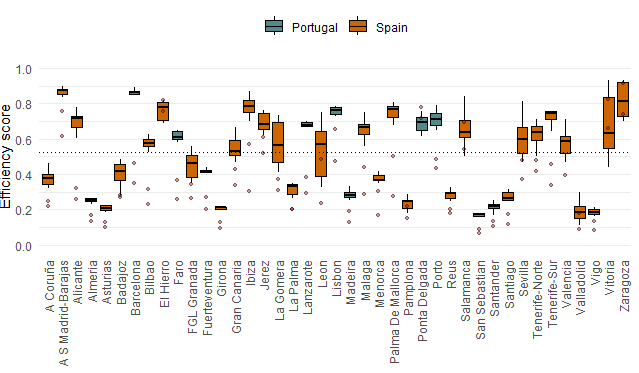
\includegraphics[width=8cm]{images/Rplot01.png}
  \vspace{-0.8cm}
  \caption{Boxplots of the bootstrapped VRS efficiency scores, for each airport.}
  \label{fig:boxplot}
\end{figure}
  \vspace{-0.3cm}

Analyzing \figref{fig:boxplot}, and considering the median value of each box, it is possible to observe
that, from the 41 airports, 24 present above average efficiencies, with Madrid-Barajas, Barcelona and
Zaragoza obtaining the highest efficiency scores, while San Sebastian, Valladolid and Vigo being the
least efficient airports. Following the airport size definition presented in Table 4.1, 16 of the 24 airports
with above average efficiency are large, while 14 of the 17 below average airports are small or medium
sized. This result suggests that larger airports tend to be more efficient. 

Considering the Portuguese airports, only Madeira airport is considered inefficient, with Lisbon being
the most efficient, followed by Porto, Ponta Delgada and Faro. The average efficiency for Portuguese
airports is 0.613, indicating that, over the period and sample considered, they are approximately 20 %
more efficient than the Spanish ones that obtained an average efficiency of 0.510.




\vspace{-0.1cm}
\subsection{Second-stage: Truncated regression }
\label{subsec:resul_trunc}

After computing the DEA efficiency scores in the first stage, a second-stage truncated regression
was conducted to address DEA’s main limitation, which is its inability to explain the effect of some
determinants in the efficiency scores. The regression was applied to the bootstrapped DEA scores, using the explanatory variables described in \tabref{tab:exp_statistics}, under the following model:

\vspace{-0.1cm}
\begin{equation}
    \label{eq:complete_regression}
\begin{aligned}
\theta_{i,t} &= \alpha + \beta_1 \text{Island}_{i} + \beta_2 \text{Military}_{i} + \beta_3 \text{Rail}_{i} \\
&\quad + \beta_4 \text{ShareCargo}_{i,t} + \beta_5 \text{ShareLCC}_{i,t} + \varepsilon_{i,t}
\end{aligned}
\end{equation}

\clearpage
\tabref{tab:regression_results} reports the coefficients and p-values for the variables considered in both the biased and
bootstrapped models. For binary variables, the coefficient represents the estimated change in the effi-
ciency score when the specific variable applies, while for continuous variables, the coefficient reflects
the marginal effect on the efficiency score of a one-unit increase in the corresponding variable \cite{simar2007}.


\begin{table}[h!]
\centering
\caption{Truncated regression results.}
\label{tab:regression_results}
\resizebox{\columnwidth}{!}{%
\begin{tabular}{l D{.}{.}{1.4} D{.}{.}{1.4} c D{.}{.}{1.4} D{.}{.}{1.4}}
    \toprule
\multirow{2}{*}{\textbf{Variable}} &\multicolumn{2}{c}{\textbf{Biased}} & \hspace{0.01cm} & \multicolumn{2}{c}{\textbf{Bootstrapped}} \\
\cmidrule{2-3} \cmidrule{5-6}
 & \multicolumn{1}{l}{\textbf{Coeff.}} & \multicolumn{1}{l}{\textbf{p-value}} && \multicolumn{1}{l}{\textbf{Coeff.}} & \multicolumn{1}{l}{\textbf{p-value}} \\
\midrule
\textit{Constant} & 0.5175 & 0.0000^{***} && 0.2602 & 0.0000^{***} \\ 
Island & 0.1858 & 0.0000^{***} && 0.1690 & 0.0000^{***} \\ 
Military & 0.0822 & 0.0578^{*} && 0.0644 & 0.0210^{**} \\ 
Rail existence & 0.4895 & 0.0000^{***} && 0.3828 & 0.0000^{***} \\ 
Share of cargo & 0.0108 & 0.0000^{***} && 0.0065 & 0.0000^{***} \\ 
Share of LCC & -0.0016 & 0.0234^{**} && 0.0007 & 0.1670 \\ 
\bottomrule
\end{tabular}%
}
\begin{flushleft}
\footnotesize
\textit{Note}: Statistically significant at 1\% $^{***}$, 5\% $^{**}$, or 10\% $^{*}$ level.
\end{flushleft}
\end{table}

\vspace{-0.5cm}
Analyzing the results, it is possible to observe that the coefficients of the variables are similar across
both models, with the bootstrapped model presenting consistently lower values. Starting by the Island
variable, its coefficient is positive and statistically significant at the 1\% significance level in both models,
indicating that airports located on islands are, on average, 18.58\% and 16.90\% more efficient than
those located on the mainland, respectively. It can also be concluded that the presence of Military operations in the airport contributes positively
on the efficiency, with a coefficient of 8.22\% in the biased model and 6.44\% in the bootstrapped one, with
the former being statistically significant at the 10\% significance level and the latter at the 5\% significance
level. Regarding the novel explanatory variable in Iberian airport studies, Rail existence, it achieved the
highest coefficient, from all variables and revealed to be statistically significant at the 1\% level, in both
models. An Iberian airport with a conventional rail connection is, on average, 48.95\% more efficient in
the biased model and 38.28\% in the bootstrapped one, respectively, than one without such a connection. Focusing on the effect the share of cargo transport has on airport efficiency, it is possible to observe
that the coefficient is positive and statistically significant at the 1\% significance level in both models,
indicating that a 1\% increase in the share of cargo, in the total WLU, results in an increase in the
efficiency score of 1.08\%, for the biased model, and 0.65\%, for the bootstrapped one. As for the share of LCC passengers, the results were inconclusive. In the biased model, the coefficient was negative and statistically significant at the 5\% significance level, suggesting that a 1\% increase
in the share of LCC passengers would lead to a 0.16\% decrease in the efficiency score. In contrast, in
the bootstrapped model, the coefficient became positive (0.07\%) but was not statistically significant.





\subsection{Dynamic Evolution: Malmquist index}
\label{subsec:resul_malm}
To complement the obtained static DEA scores, the Malmquist Productivity Index
(MPI) was applied to analyze how the productivity of each Iberian airport evolved over the considered
period (2016-2023). The dynamic evaluation that this methodology offers becomes especially important
for a period that includes an external shock as the COVID-19 pandemic, since it allows for a better
understanding of the impact of such events in airport performance, not only in the affected years (in this
case 2020 and 2021), but also in the subsequent recovery years.

\tabref{tab:malmquist_summary} presents the geometric means of the MPI for the Iberian airports, as well as the four components it can be decomposed into: Technological Change (TECHC), Efficiency Change (EC), which is further divided into Pure Efficiency Change (PEC) and Scale Efficiency Change (SEC). Two additional notes must be done: first, the MPI calculations were made without accounting for the bias present in
the DEA scores, i.e., no bootstrapping technique was applied, as no function in the softwares (RStudio
and Stata) used is readily available. Second, 4 of the initial 41 airports do not present the results of
the decomposition of EC, due to failure in the estimation of PEC (that is obtained by conducting a MPI
analysis under VRS), namely for the airports El Hierro, La Gomera, Leon and Ponta Delgada.


Analyzing \tabref{tab:malmquist_summary}, it is possible to observe that, on average, Iberian airports experienced a productivity growth of 3.82\% over the period considered, with 37 out of the 41 airports showing improvement (MPI > 1). The main driver of this productivity growth was Efficiency Change (EC), which increased by 3.27\%, while Technological Change (TECHC) contributed with a smaller increase of 0.58\%. This result indicates that most of the productivity growth was due to improvements in how efficiently airports utilized their resources, rather than advancements in technology or infrastructure. An expected result is that the highest values of Technological Change (TECHC) are concentrated in
the largest airports as Madrid-Barajas, Barcelona, Lisbon, Porto and Valencia, with values ranging from
1.0367 to 1.0848. When analyzing the decomposition of EC, it is possible to observe that the average Pure Efficiency
Change (PEC) increased by 2.96\%, while Scale Efficiency Change (SEC) slightly decreased by 0.24\%.
This suggests that most of the efficiency improvements were due to better management and operational
practices, rather than changes in the scale of operations.
\clearpage
%\renewcommand{\arraystretch}{0.9}
\begin{table}[t!]
\centering
\caption{Geometric mean of Malmquist Productivity Index (MPI) and its components for each airport} 
\label{tab:malmquist_summary}
\resizebox{\columnwidth}{!}{%
\begin{tabular}{lccccc}
  \toprule
  \textbf{Airport} & \textbf{MPI} & \textbf{TECHC} & \textbf{EC} & \textbf{PEC} & \textbf{SEC} \\
  \midrule
A Coruña & 1.0096 & 0.9863 & 1.0236 & 1.0317 & 0.9922 \\
A S Madrid-Barajas & 1.0486 & 1.0566 & 0.9924 & 1.0000 & 0.9924 \\
Alicante-Elche & 1.0238 & 1.0331 & 0.9910 & 0.9931 & 0.9980 \\
Almería & 1.0007 & 0.9792 & 1.0219 & 1.0277 & 0.9944 \\
Asturias & 1.0660 & 0.9945 & 1.0718 & 1.0819 & 0.9907 \\
Badajoz & 1.1119 & 1.0094 & 1.1016 & 1.1970 & 0.9203 \\
Barcelona & 1.0420 & 1.0848 & 0.9605 & 1.0000 & 0.9605 \\
Bilbao & 1.0173 & 0.9841 & 1.0337 & 1.0118 & 1.0216 \\
El Hierro &1.0462 & 0.9812 & 1.0662 &  &  \\  
Faro & 0.9550 & 0.9920 & 0.9627 & 0.9898 & 0.9726 \\
FGL Granada & 0.9974 & 0.9758 & 1.0221 & 1.0187 & 1.0033 \\
Fuerteventura & 1.0126 & 1.0067 & 1.0059 & 0.9961 & 1.0098 \\
Girona & 1.0006 & 0.9940 & 1.0067 & 1.0054 & 1.0012 \\
Gran Canaria & 1.0459 & 1.0196 & 1.0258 & 1.0196 & 1.0060 \\
Ibiza & 1.0240 & 1.0069 & 1.0170 & 1.0136 & 1.0033 \\
Jerez & 1.0107 & 1.0107 & 1.0000 & 1.0000 & 1.0000 \\
La Gomera &1.1073& 0.9764& 1.1341 &  &  \\ 
La Palma & 1.0282 & 0.9940 & 1.0345 & 1.0334 & 1.0011 \\
Lanzarote & 1.0269 & 1.0079 & 1.0189 & 1.0174 & 1.0014 \\
Leon & 1.1234 & 0.9938 & 1.1305 &  &  \\
Lisbon & 1.0566 & 1.0566 & 1.0000 & 1.0000 & 1.0000 \\
Madeira & 1.0393 & 1.0159 & 1.0230 & 1.0296 & 0.9936 \\
Malaga & 1.0435 & 1.0184 & 1.0247 & 0.9964 & 1.0284 \\
Menorca & 1.0160 & 0.9965 & 1.0196 & 1.0165 & 1.0030 \\
Palma de Mallorca & 1.0253 & 1.0400 & 0.9858 & 0.9976 & 0.9882 \\
Pamplona & 1.0468 & 0.9929 & 1.0543 & 1.0683 & 0.9869 \\
Ponta Delgada & 1.0512& 1.0300 & 1.0205 &  &  \\
Porto & 1.0595 & 1.0595 & 1.0000 & 1.0000 & 1.0000 \\
Reus & 1.0341 & 0.9788 & 1.0565 & 1.0583 & 0.9983 \\
Salamanca & 0.9863 & 0.9829 & 1.0034 & 1.0000 & 1.0034 \\
San Sebastián & 1.0229 & 0.9781 & 1.0459 & 1.0465 & 0.9995 \\
Santiago & 1.0438 & 0.9881 & 1.0564 & 1.0548 & 1.0015 \\
Santander & 1.0557 & 0.9838 & 1.0731 & 1.0855 & 0.9887 \\
Sevilla & 1.0436 & 0.9983 & 1.0454 & 1.0366 & 1.0084 \\
Tenerife Norte & 1.0305 & 1.0214 & 1.0089 & 1.0114 & 0.9975 \\
Tenerife-Sur & 0.9818 & 0.9988 & 0.9830 & 0.9760 & 1.0072 \\
Valencia & 1.1265& 1.0367 & 1.0866 &1.0600 & 1.0251 \\
Valladolid & 1.0799 & 0.9704 & 1.1128 & 1.1165 & 0.9967 \\
Vigo & 1.0230 & 0.9823 & 1.0415 & 1.0446 & 0.9970 \\
Vitoria & 1.1004 & 1.0191 & 1.0797 & 1.0598 & 1.0188 \\
Zaragoza & 1.0031 & 1.0031 & 1.0000 & 1.0000 & 1.0000 \\
 \midrule
 Mean & 1.0382
 & 1.0058  
 & 1.0327
 &1.0296
 & 0.9976
 \\
 \midrule
\end{tabular}%
}
\end{table}


The best performing airports in the considered period were Badajoz, Leon and Valencia. The latter
achieved the highest MPI, with a value of 1.1265, indicating a significant productivity growth of 12.65\%.
This growth was mainly driven by a strong increase in EC (8.66\%), with both PEC and SEC contributing
positively to the efficiency change. Leon and Badajoz also showed strong performance, with MPIs of
1.1234 and 1.1119, respectively, driven by improvements in efficiency rather than advancements of the
frontier. Unfortunately, for Leon the decomposition of EC cannot be analyzed but for Badajoz, unlike
Valencia a decrease of 7.87\% in the scale efficiency was registered.

As previously said, 4 airports presented a decrease in efficiency, namely Faro, FGL Granada, Sala-
manca and Tenerife-Sur. Faro had the lowest MPI, with a value of 0.9550, indicating a productivity
decline of 4.50\%. This result is explained by a decrease in TECHC (0.80\%) and EC (3.73\%), with both
PEC and SEC contributing negatively to the efficiency change result. FGL Granada also experienced a
slight decline in productivity, with an MPI of 0.9974, driven by a decrease in TECHC (2.42\%) despite the
increase in EC (2.21\%). Salamanca and Tenerife-Sur had similar MPI results, with values of 0.9863 and
0.9818, respectively. Both airports experienced declines in TECHC (1.71\% and 0.12\%, respectively)
while for EC, Salamanca had a slight increase (0.34\%) and Tenerife-Sur a decrease (1.70\%). Also, both
airports presented an improvement in scale.

To better understand how the MPI changed and what caused its variations along the years, \figref{fig:malmquist}
displays the evolution of the average MPI and its components for each year. The score of each year
represents the change in relation to the previous year. To provide the starting point representation, the
first year 2016, was also added, so all the components under study have a value equal to one in this
year.
\vspace{-0.5cm}
\begin{figure}[H]
  \centering
  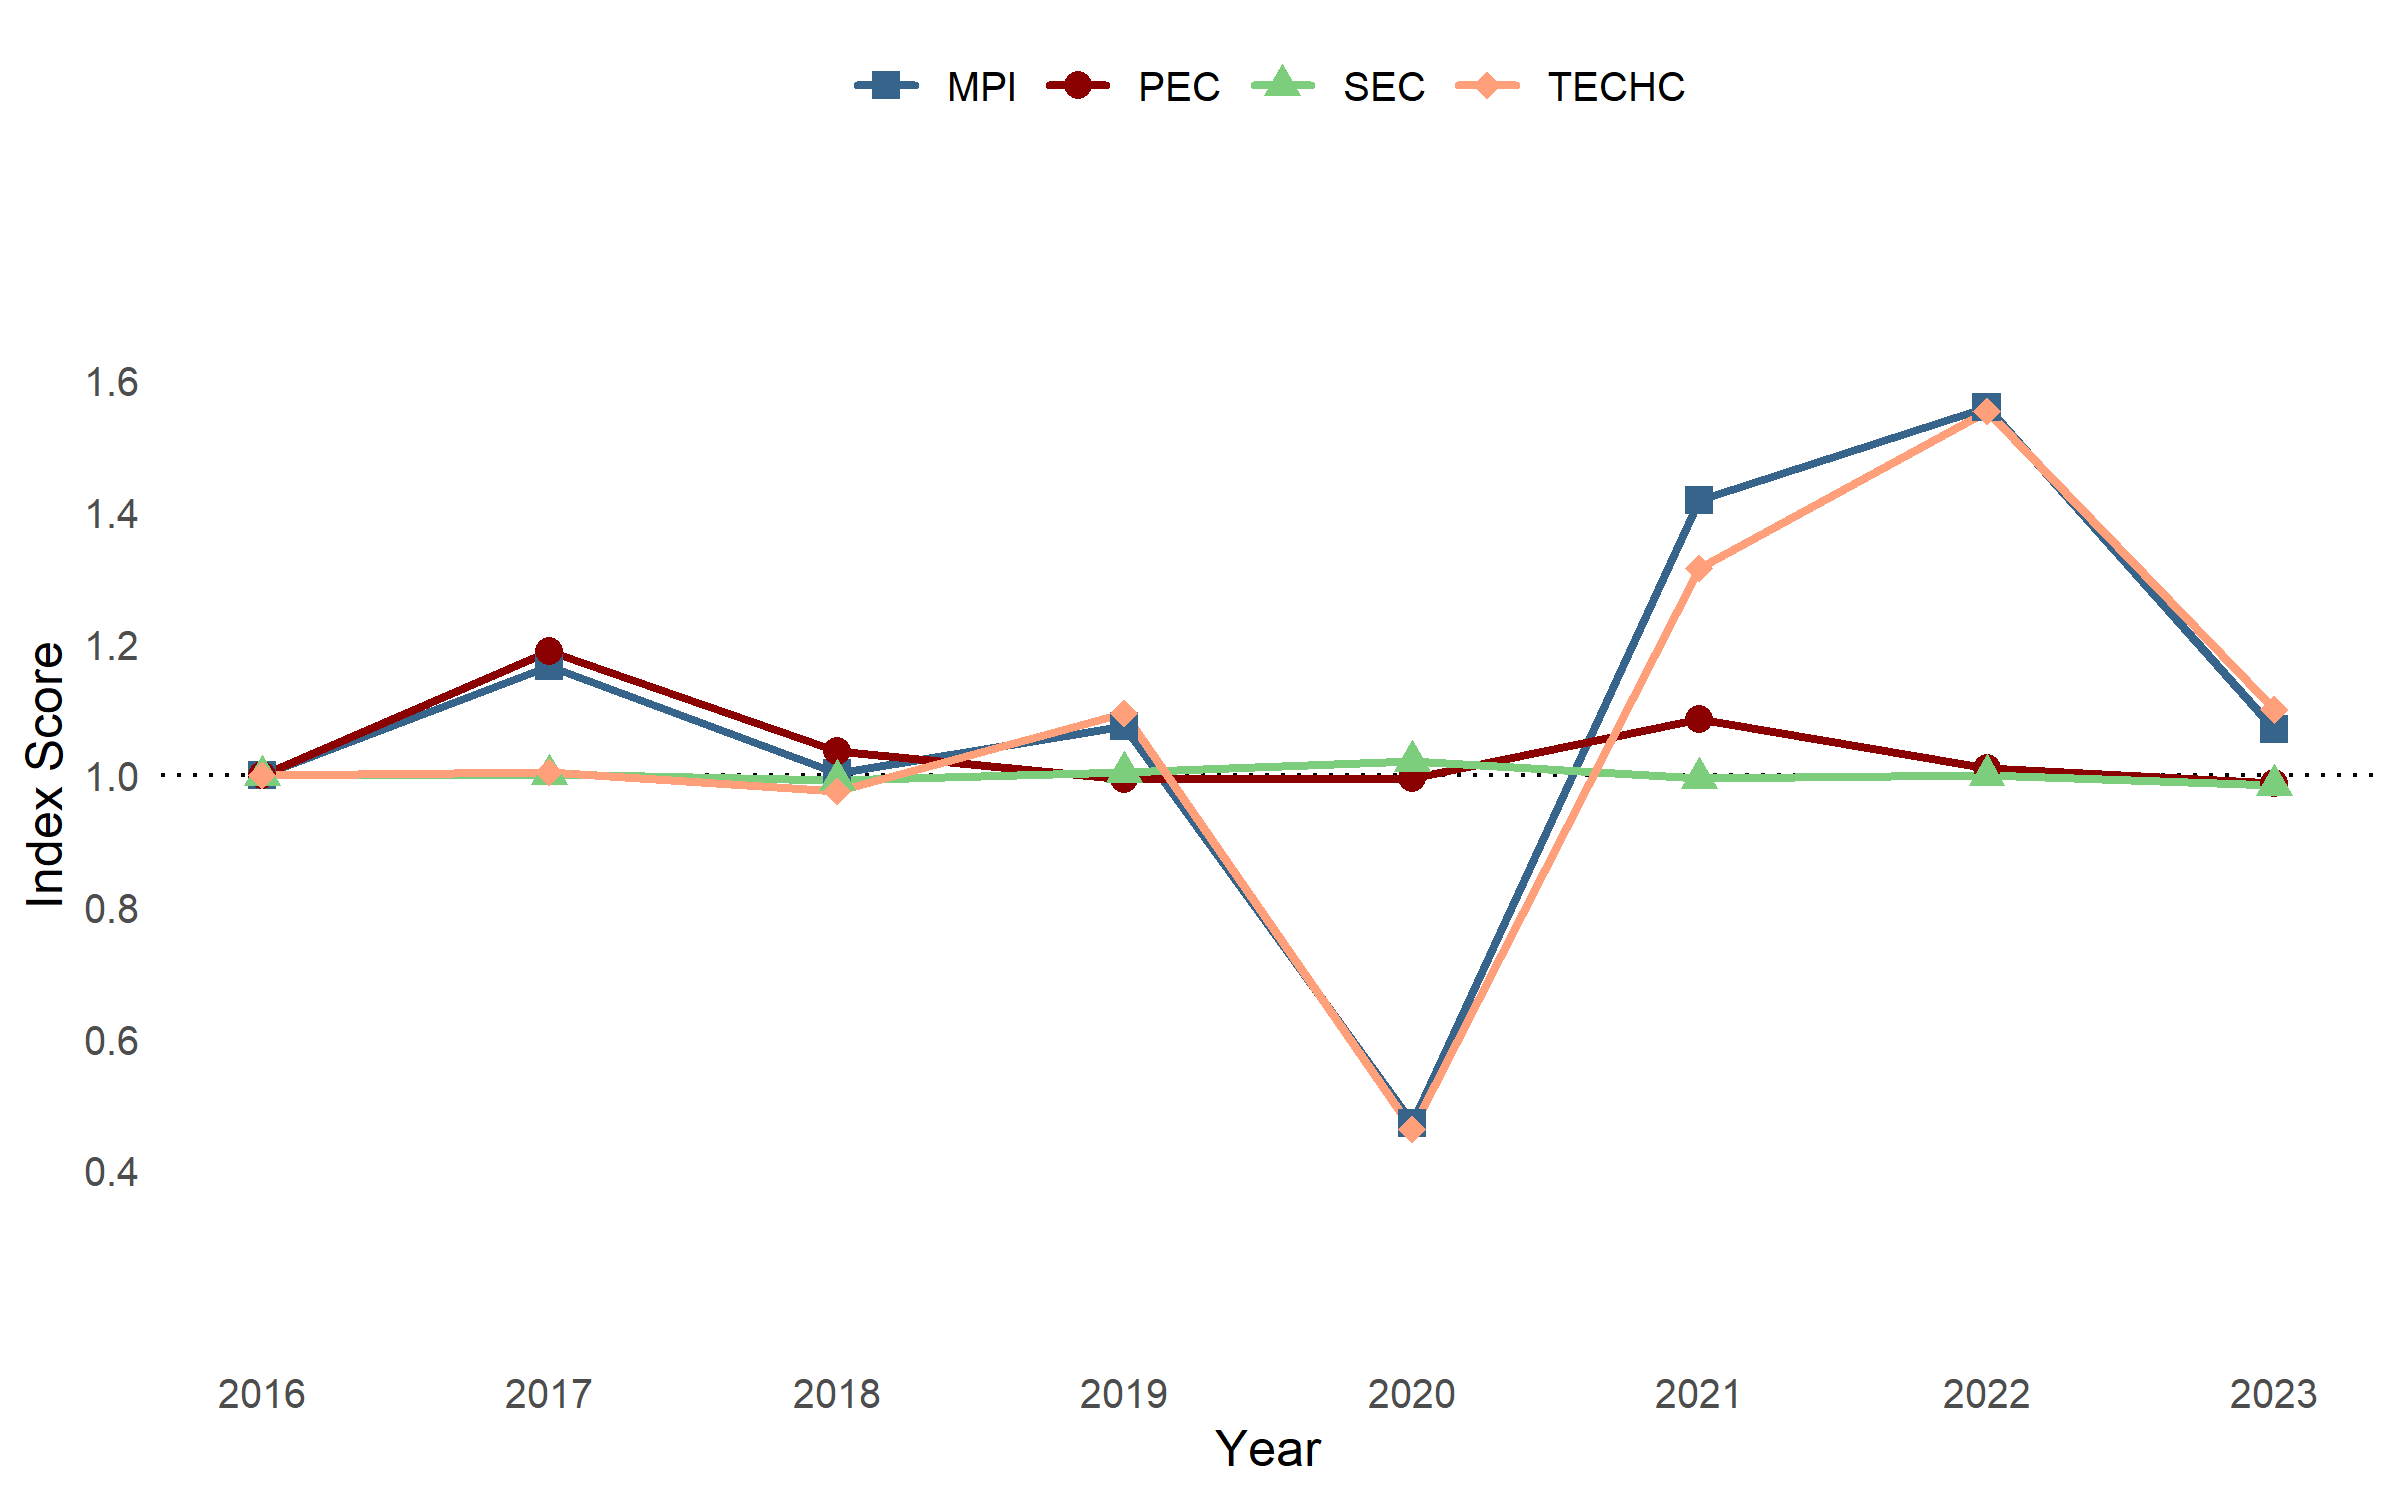
\includegraphics[width=8cm]{images/malmquist_plot.png}
  \vspace{-0.5cm}
  \caption{Average of Malmquist Productivity Index (MPI) and its components for each year}
  \label{fig:malmquist}
\end{figure}
\vspace{-0.5cm}

Analyzing \figref{fig:malmquist}, it is possible to observe that the average MPI was above 1 in all years, except
for 2020. The overall trend for each component of the MPI can also be examined. TECHC represented
the principal contributor for MPI fluctuations, while PEC and SEC showed a more constant evolution,
with SEC remaining almost unchanged through the whole period and being the only component with an
average value below 1. In the first years, the MPI had two years with different growth patterns. In 2017, the MPI reached a
value of 1.1657 associated with an improvement in PEC, while TECHC remained practically constant.
However in 2019, MPI growth, with a value of 1.0748, was mainly driven by an increase in TECHC.
From 2019 to 2020, an expected decline in TECHC caused the MPI to drop to a value of 0.4719, the
lowest in the period. However, observing the subsequent years it can be concluded that the Iberian
airports managed to recover well from the severe impact caused by the COVID-19, which lead to a
positive average of the MPI in the considered time period. It is important to note that, in 2021 both
TECHC and PEC increased, with PEC achieving its second highest score of 1.0852. A rise in TECHC
was expected, but this result in PEC indicates that, despite the challenging circumstances, airports were
able to improve their efficiency through better management of their resources.
%%%%%%%%%%%%%%%%%%%%%%%%%%%%%%%%%%%%%%%%%%%%%%%%%%%%%%%%%%%%%%%%%%%%%%

%\begin{table}[!h]
 %\begin{center}
  %  \begin{tabular}{lccc}
   %   Model           & $C_L$ & $C_D$ & $C_{M y}$ \\
    %  \hline
  %    Euler           & 0.083 & 61,652,021  & -0.110    \\
   %   Navier--Stokes  & 0.078 & 0.023 & -0.101    \\
    %  \hline
    %\end{tabular}
  %\end{center}
  %\caption[Table caption shown in TOC]{Table caption}
  %\label{table:simple}
%\end{table}
